\newpage
\chapter{Nombres Complexes}
\vspace{3mm} %5mm vertical space
\section{Conversion polaire - cartésienne}
\vspace{3mm} %5mm vertical space

Définition du module: \\

le module noté $|Z|$ est la longueur du segment (rayon). Elle peut être mesurée  grâce à la formule de pythagore ($\sqrt{a²+b²}$). \\


\vspace{5mm} %5mm vertical space
Représentation Géographique \\

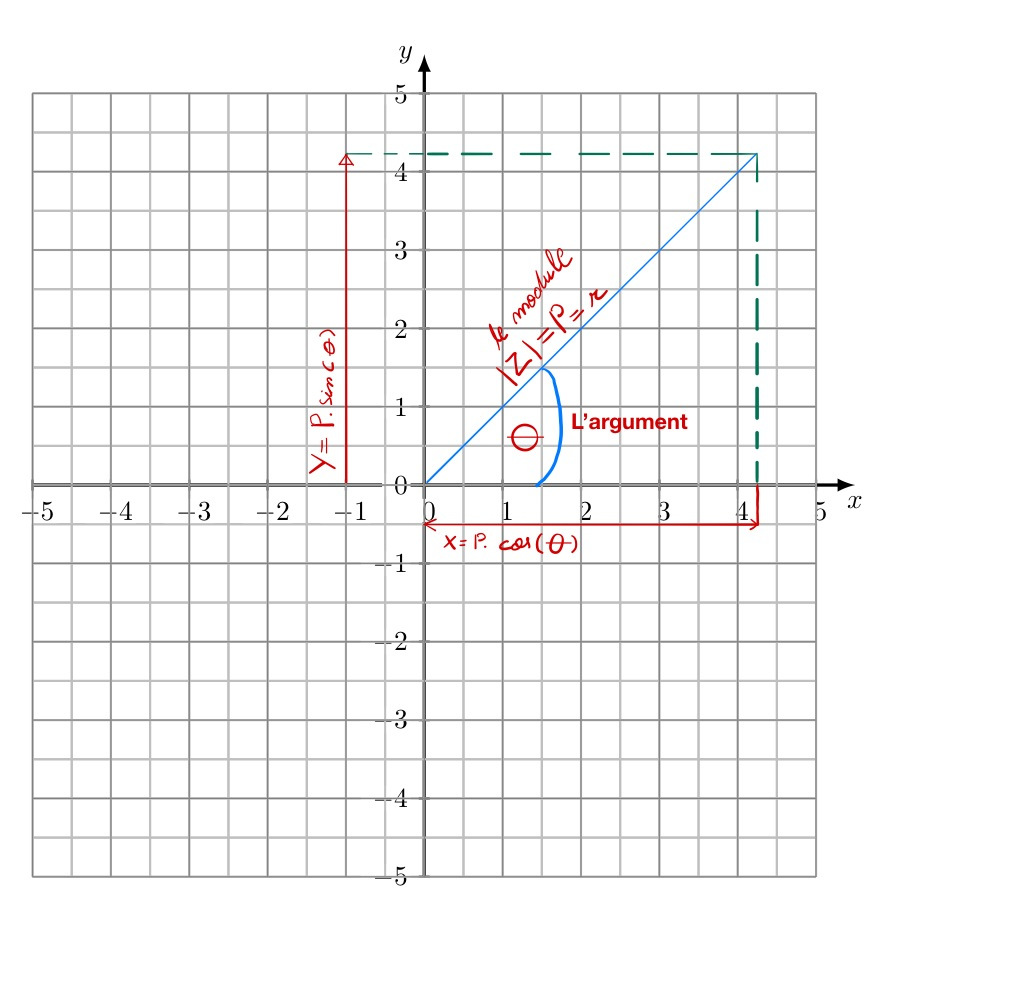
\includegraphics[scale=1.5]{cart-mod}
\vspace{2mm} %5mm vertical space

Démonstration : \\

$|Z| = \rho cos(\theta)+ \rho sin(\theta) *i$ \\
$|Z| = \sqrt(\rho^{2} cos(\theta)^{2}+ \rho^{2} sin(\theta)^{2})$ \\
$|Z| = \sqrt(\rho^{2} cos(\theta)^{2}+ sin(\theta))*i $ \\
$|Z| = \sqrt(\rho^{2}) $ \\
$|Z| = \rho $ \\

$\rho$ est le module et $\theta$ est l'argument \\
$Z= P(cos(\theta) + sin(\theta)*i )$ ou $Z= P(cis(\theta))$\\

\newpage

\section{Conversion Cartésienne - Polaire}
\vspace{3mm} %5mm vertical space

$\rho$ = $\sqrt(x²+y²)$ \\

Démonstration Géométriquement $\theta$ \\

Nous pouvons voir que $\theta$ est modifié en fonction de X et de Y que si nous dessinons un cercle, nous pouvons voir que le segment Y est une tangeante au cercle de rayon X. \\

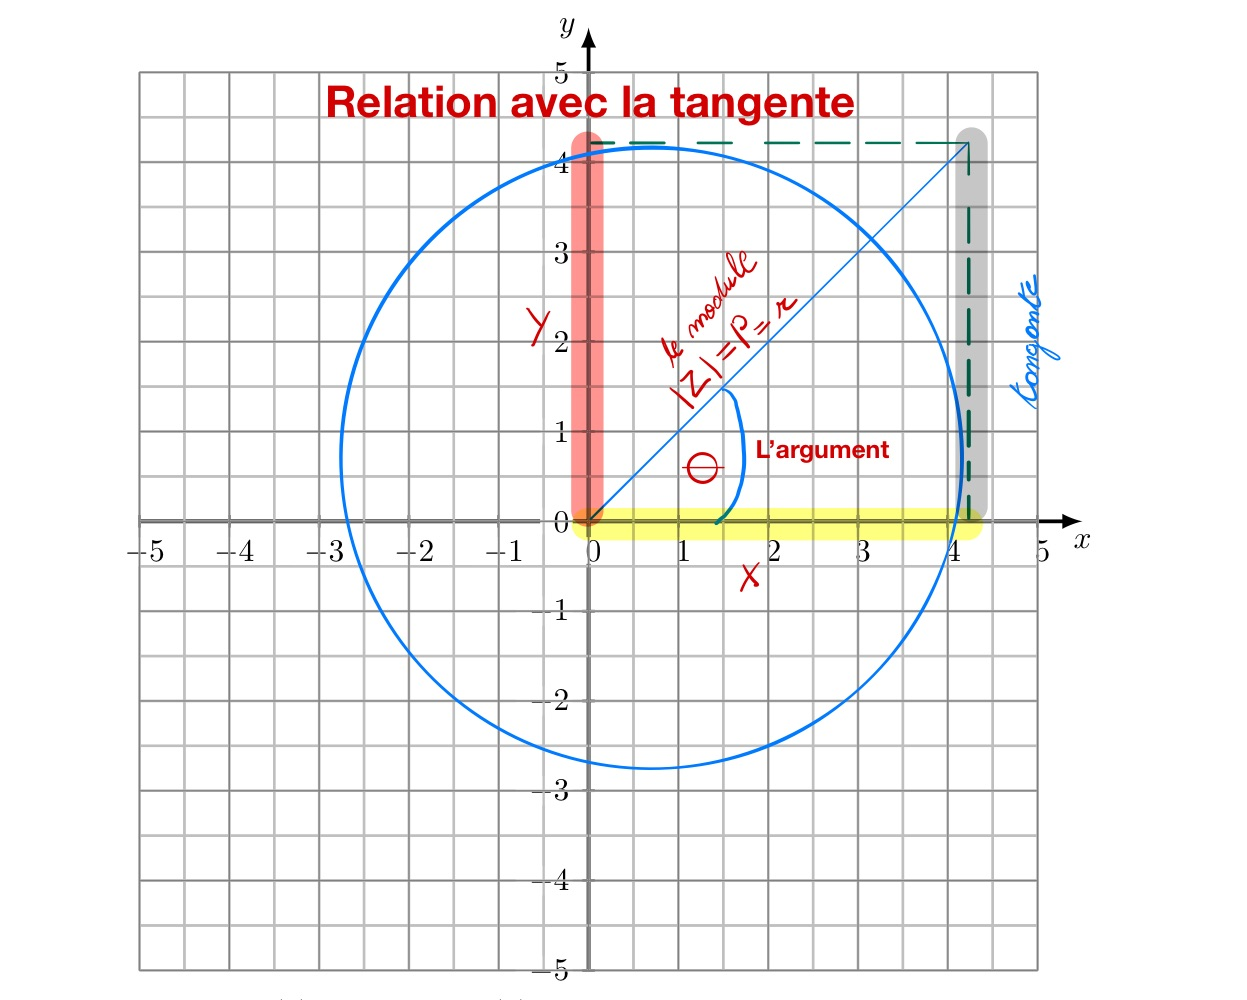
\includegraphics[scale=0.3]{cart-tg}

$X=\rho * cos(\theta)$ $ $ $ Y=\rho * sin(\theta)$

\vspace{5mm} %5mm vertical space
Démonstration Algébriquement $\theta$ \\

$\frac{Y}{X}$ = $\frac{\rho * sin(\theta)}{\rho * cos(\theta)}$ \\
$\frac{Y}{X}$ = $\frac{sin(\theta)}{cos(\theta)}$ \\
$\frac{Y}{X}$ = tg($\theta)$ \\

\vspace{5mm} %5mm vertical space
Conclusion : \\

$\theta = arctg(\frac{Y}{X})$ \\

$tg(\theta) = \frac{Y}{X}$


\newpage

\section{Conversion exponentielle - cartésienne}
\vspace{3mm} %5mm vertical space




\section{Nombre Complexes addition}
\vspace{3mm} %5mm vertical space



\section{Nombre Complexes soustraction}
\vspace{3mm} %5mm vertical space



\section{Nombre Complexes multiplication}
\vspace{3mm} %5mm vertical space



\section{Nombre Complexes division}
\vspace{3mm} %5mm vertical space
